\documentclass[a4paper,16pt]{article}
\usepackage[margin=0.8in]{geometry}
\usepackage{sectsty}
\sectionfont{\Huge\bfseries}
\subsectionfont{\huge\bfseries}
\usepackage{courier}
\usepackage{caption}
\captionsetup{font=large,labelfont=large}
\usepackage{graphicx}
\usepackage{listings}
\usepackage{subcaption}
\usepackage{setspace}
\usepackage{fancyhdr}
\usepackage{lastpage}
\pagestyle{fancy}
\fancyfoot{} % clear all footer fields
\fancyfoot[LE,RO]{\thepage}           % page number in "outer" position of footer line
\fancyfoot[RE,LO]{} % other info in "inner" position of footer line
\rfoot{Page \thepage \hspace{1pt} of \pageref{LastPage}}
\lstset{language=Matlab,
	basicstyle=\ttfamily\Large,
	numbers=left,
	tabsize=1,
	stepnumber=1,
	breaklines=true,
	frame=single,
	xleftmargin=19pt,
	keywords={imread,rgb2gray,for,end,plot,imshow,imtool,size,zeros,imwrite,subplot,double,uint8,title,max,min,abs}}
\usepackage{tocloft}
\renewcommand\cftsecfont{\LARGE}
\renewcommand\cftsecpagefont{\LARGE}
\renewcommand\cftsecafterpnum{\par\addvspace{6pt}}

\begin{document}
	{
		
		\doublespacing
		
		\pagenumbering{arabic}
		{
			\renewcommand\contentsname{\Huge Contents}
			\renewcommand\cftsubsecfont{\large}
			
			\doublespacing
			\tableofcontents
			\addtocontents{toc}{~\hfill\textbf{\LARGE Page}\par}
		}
	}
	\newpage
	
	\section{Assignment 1}
	\vspace{0.2in}
	\subsection{Negative of an image}
	\indent	\lstinputlisting{negate.m}
	\vspace{1in}
	\begin{figure}[h!]
		\begin{subfigure}[h]{0.4\linewidth}
			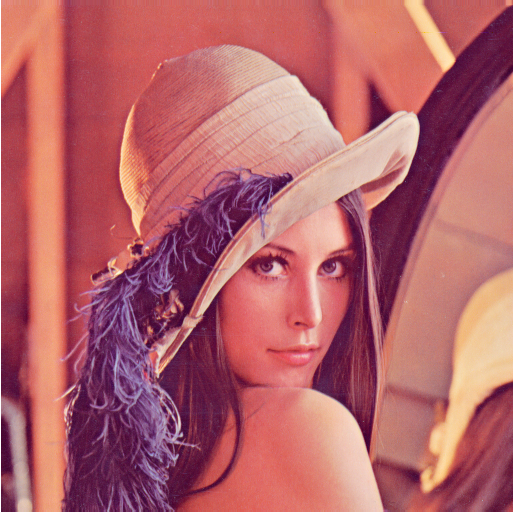
\includegraphics[width=\linewidth]{original}
			\caption{Original Image}
		\end{subfigure}
		\hfill
		\begin{subfigure}[h]{0.4\linewidth}
			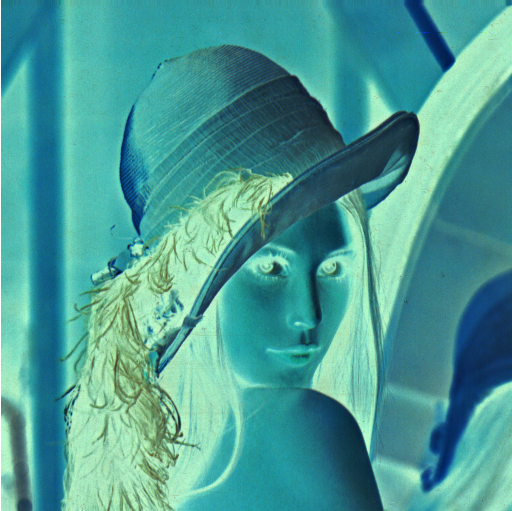
\includegraphics[width=\linewidth]{negative}
			\caption{Negative Image}
		\end{subfigure}%
		\caption{a normal and a negative image}
	\end{figure}
	\newpage
	\section{Assignment 2}
	\vspace{0.2in}
	\subsection{Plotting the histogram of an image}
	\vspace{0.2in}
		\lstinputlisting{his.m}
		\vspace{1.4in}
		\begin{figure}[h!]
			\begin{subfigure}[h]{0.4\linewidth}
				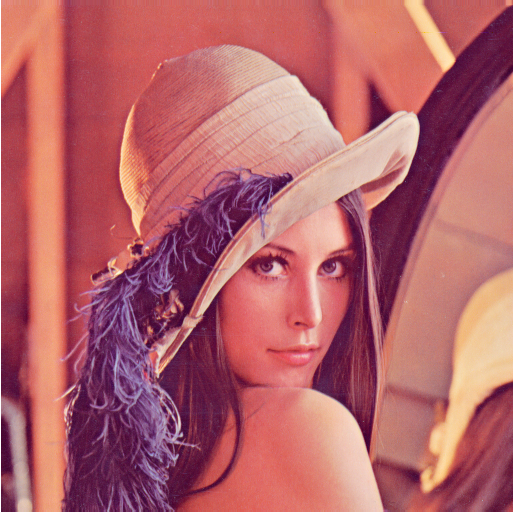
\includegraphics[scale=0.45,height=0.9\linewidth]{original}
				\caption{Original Image}
			\end{subfigure}
			\hfill
			\begin{subfigure}[h]{0.57\linewidth}
				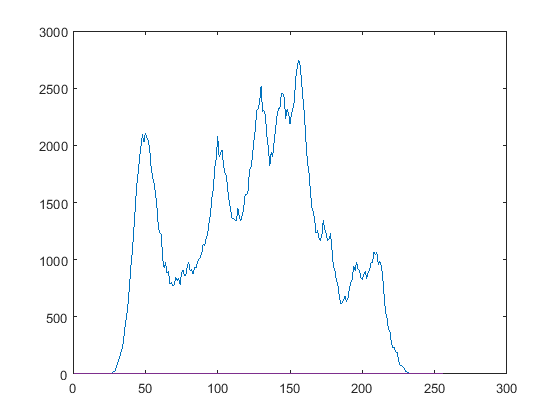
\includegraphics[width=\linewidth]{histogram}
				\caption{Histogram of the Image}
			\end{subfigure}%
			\caption{Image \& histogram of the image}
		\end{figure}
	\newpage
	\subsection{Histogram equalization}
	\vspace{0.3in}
	\lstinputlisting{histequal.m}
	\newpage
	
	\begin{figure}[h!]
		\begin{subfigure}[h]{0.62\linewidth}
			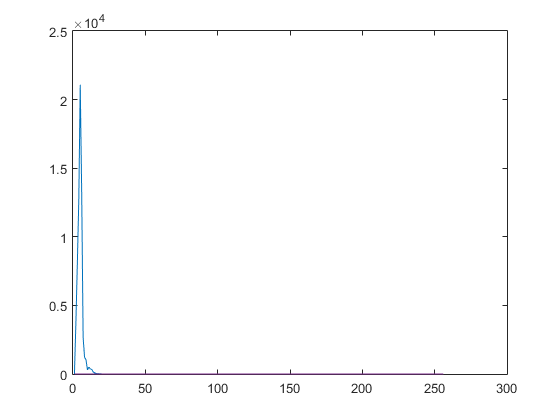
\includegraphics[width=0.82\linewidth,scale=0.3,height=0.5\linewidth]{hist1}
			\caption{Original Histogram}
		\end{subfigure}
		\begin{subfigure}[h]{0.62\linewidth}
			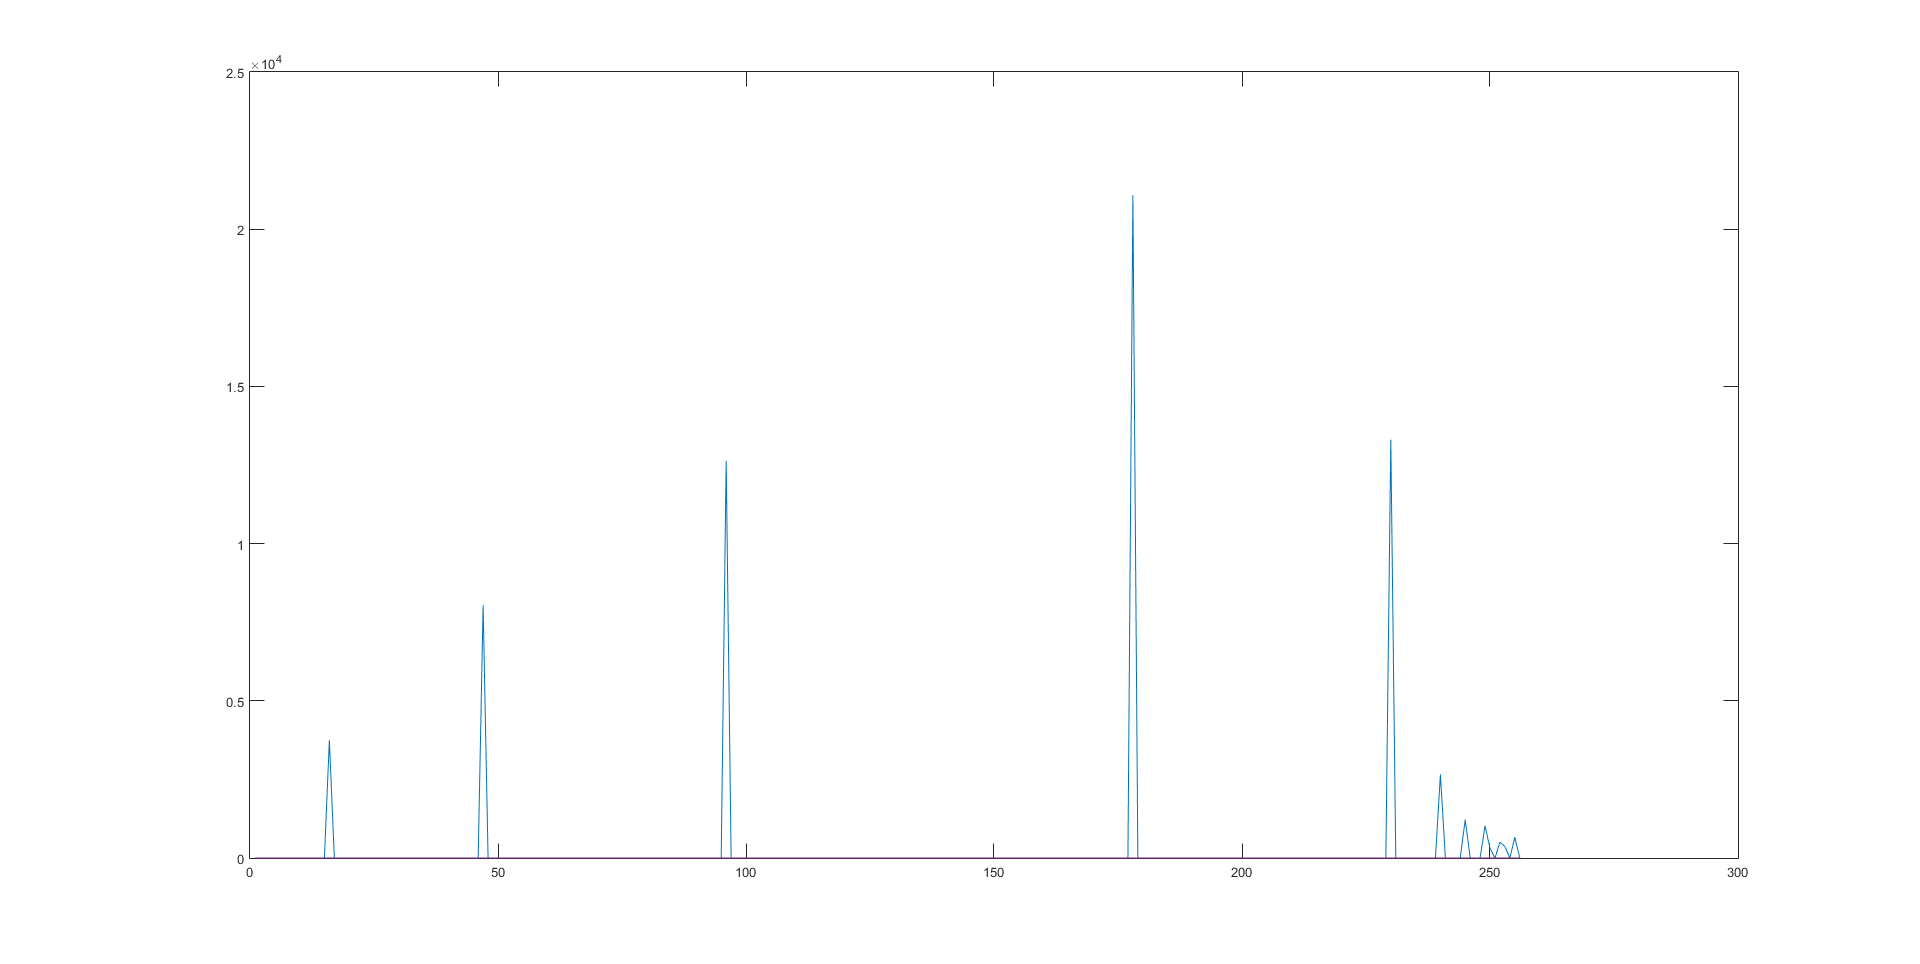
\includegraphics[scale=0.4,width=0.8\linewidth,height=0.5\linewidth]{hist2}
			\caption{Histogram after equalization}
		\end{subfigure}%
		\caption{Histograms of the images}
	\end{figure}
	\begin{figure}[h!]
		\begin{subfigure}[h]{0.6\linewidth}
			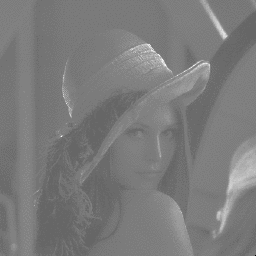
\includegraphics[scale=1]{Lenna}
			\caption{Original Low contrast Image}
		\end{subfigure}
		\hfill
		\begin{subfigure}[h]{0.6\linewidth}
			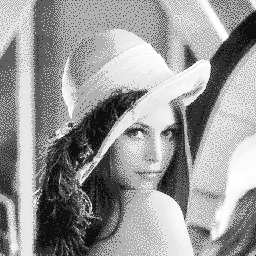
\includegraphics[scale=0.76]{myGray}
			\caption{Equalized image}
		\end{subfigure}%
		\caption{Image \& histogram of the image}
	\end{figure}
	\section{Assignment 3}
	\subsection{Mean Filter}
	\lstinputlisting{fil.m}
	\begin{figure}[b!]
		\begin{subfigure}[h]{0.45\linewidth}
			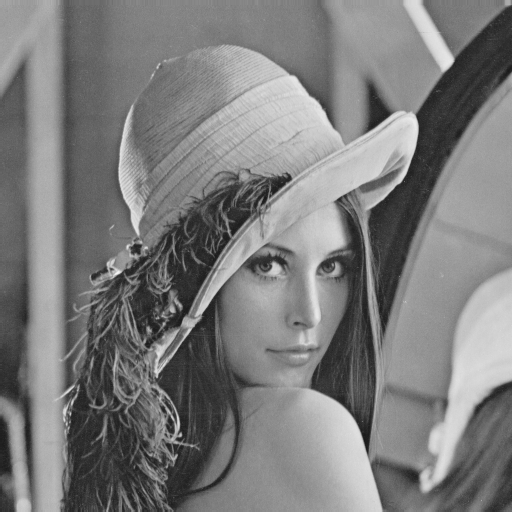
\includegraphics[width=\linewidth]{grayscale}
			\caption{Original Image}
		\end{subfigure}
		\hfill
		\begin{subfigure}[h]{0.45\linewidth}
			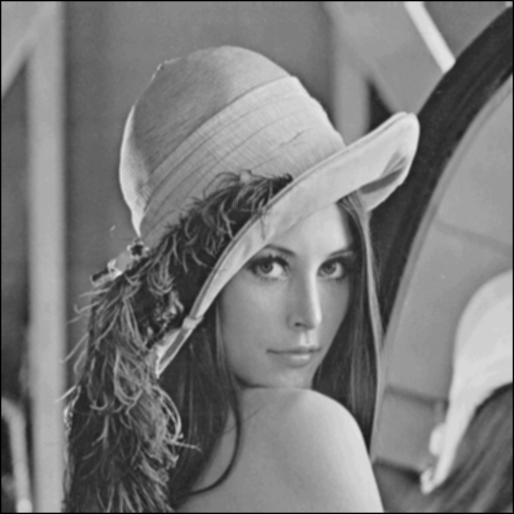
\includegraphics[width=\linewidth]{meanfilter}
			\caption{Mean filtered image}
		\end{subfigure}%
		\caption{Normal \& Filtered Image}
	\end{figure}
	\newpage
	\subsection{Median Filter}
	\vspace{0.2in}
	\lstinputlisting{medfilter.m}
	\begin{figure}[h!]
		\begin{subfigure}[h]{0.45\linewidth}
			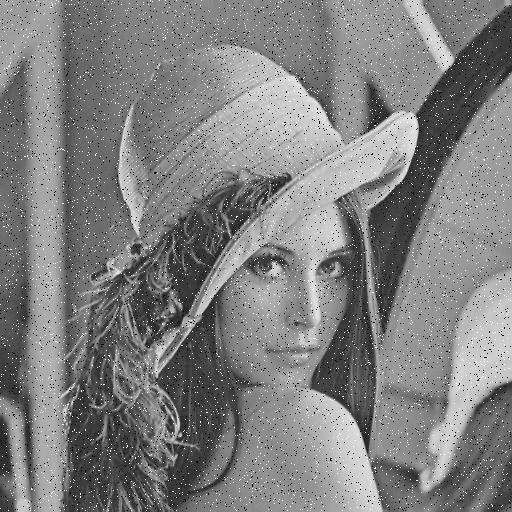
\includegraphics[width=\linewidth]{salt}
			\caption{Original Image}
		\end{subfigure}
		\hfill
		\begin{subfigure}[h]{0.45\linewidth}
			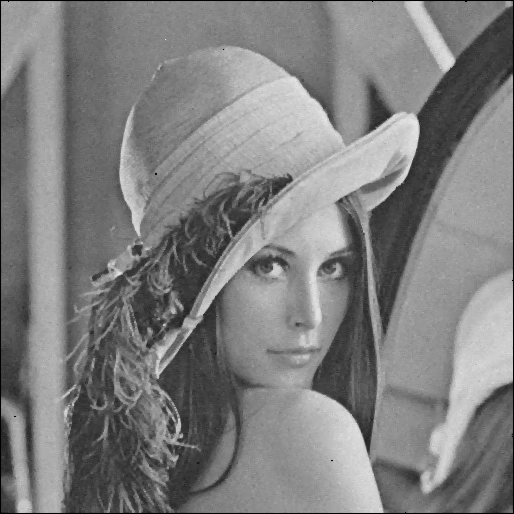
\includegraphics[width=\linewidth]{medianfilt}
			\caption{Median filtered image}
		\end{subfigure}%
		\caption{Noisy \& Filtered Image}
	\end{figure}
	\newpage
	\subsection{Min \& Max  Filter}
	\vspace{0.05in}
	\lstinputlisting{maxminfilter.m}
	\vspace{0.2in}
	\begin{figure}[h!]
		\begin{subfigure}[h!]{0.3\linewidth}
			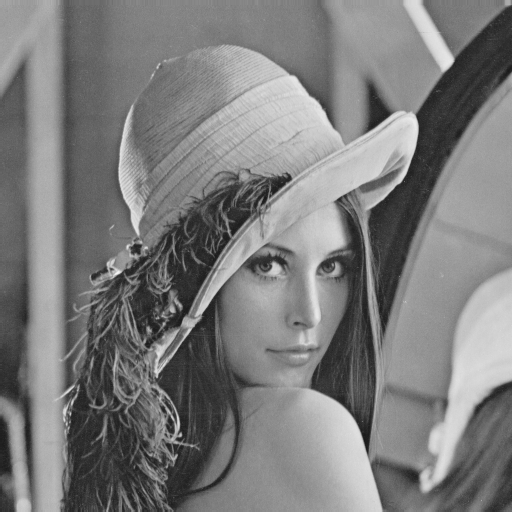
\includegraphics[width=\linewidth]{grayscale}
			\caption{Original grayscale image}
		\end{subfigure}
		\hfill
		\begin{subfigure}[h!]{0.3\linewidth}
			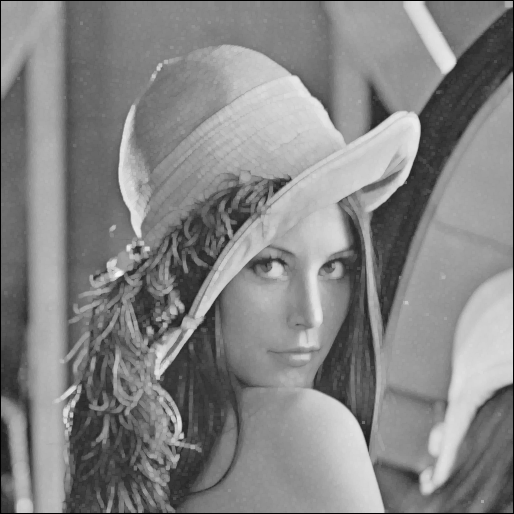
\includegraphics[width=\linewidth]{maxfilter}
			\caption{Max filtered Image}
		\end{subfigure}
		\hfill
		\begin{subfigure}[h!]{0.3\linewidth}
			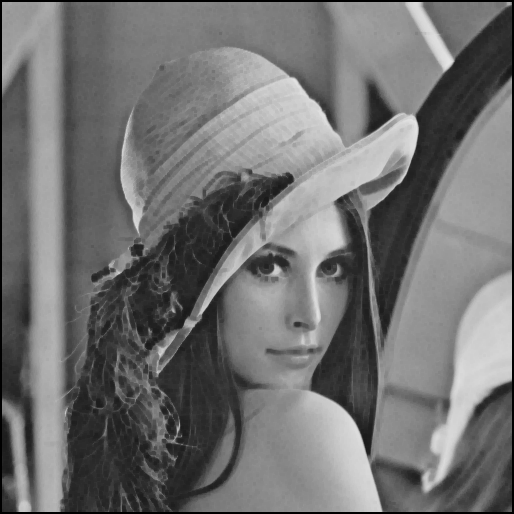
\includegraphics[width=\linewidth]{minfilter}
			\caption{Min filtered Image}
		\end{subfigure}%
		\caption{Min \& Max Filtered Images}
	\end{figure}
	\newpage
	\section{Assignment 4}
	\vspace{0.2in}
	\subsection{Edge Detection}
	\vspace{0.2in}
	\lstinputlisting{edge.m}
	\vspace{0.4in}
	\begin{figure}[h!]
		\begin{subfigure}[h!]{0.45\linewidth}
			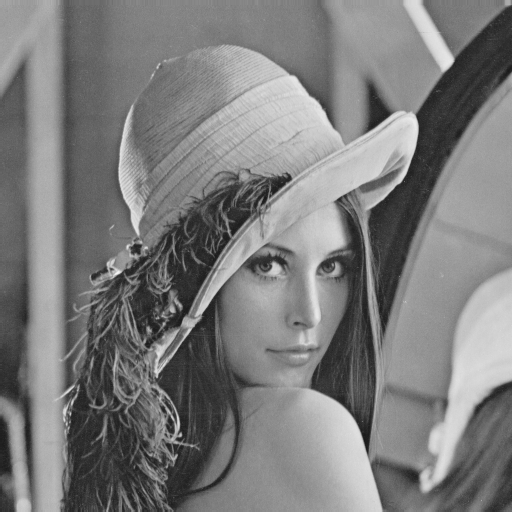
\includegraphics[width=\linewidth]{grayscale}
			\caption{Original grayscale image}
		\end{subfigure}
		\hfill
		\begin{subfigure}[h!]{0.45\linewidth}
			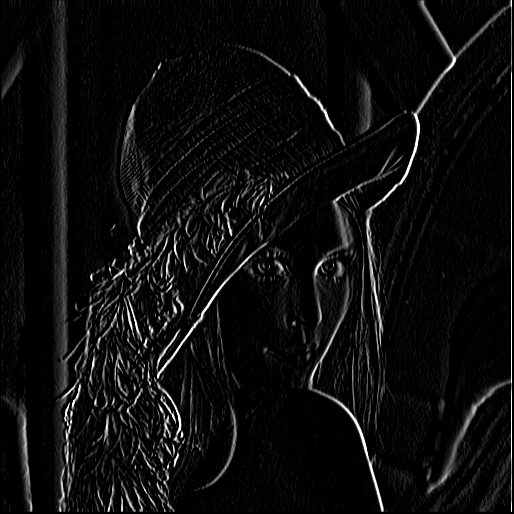
\includegraphics[width=\linewidth]{horizontal}
			\caption{Horizontal edge}
		\end{subfigure}
		\hfill
		\centering
		\begin{subfigure}[h!]{0.45\linewidth}
			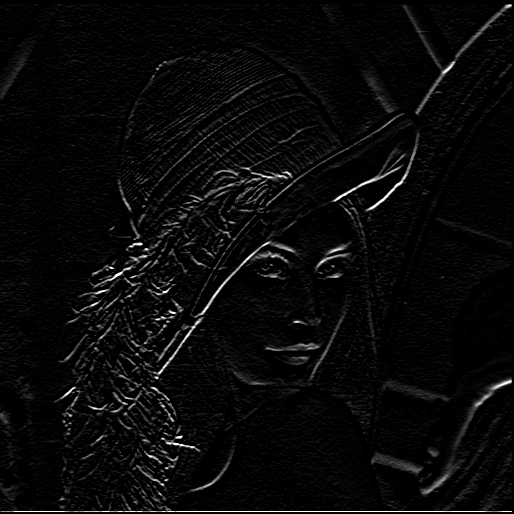
\includegraphics[width=\linewidth]{vertical}
			\caption{Vertical edge}
		\end{subfigure}%
		\caption{Min \& Max Filtered Images}
	\end{figure}
	\newpage
	
	\subsection{Segmentation}
	\vspace{0.2in}
	\lstinputlisting{segmentation.m}
	\vspace{0.8in}
	\begin{figure}[h!]
		\begin{subfigure}[h!]{0.45\linewidth}
			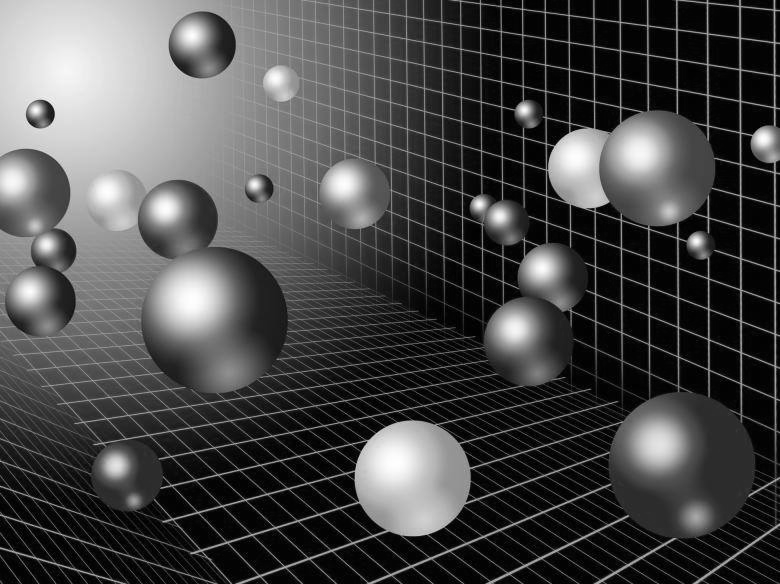
\includegraphics[width=\linewidth]{ballg}
			\caption{Original grayscale image}
		\end{subfigure}
		\hfill
		\begin{subfigure}[h!]{0.45\linewidth}
			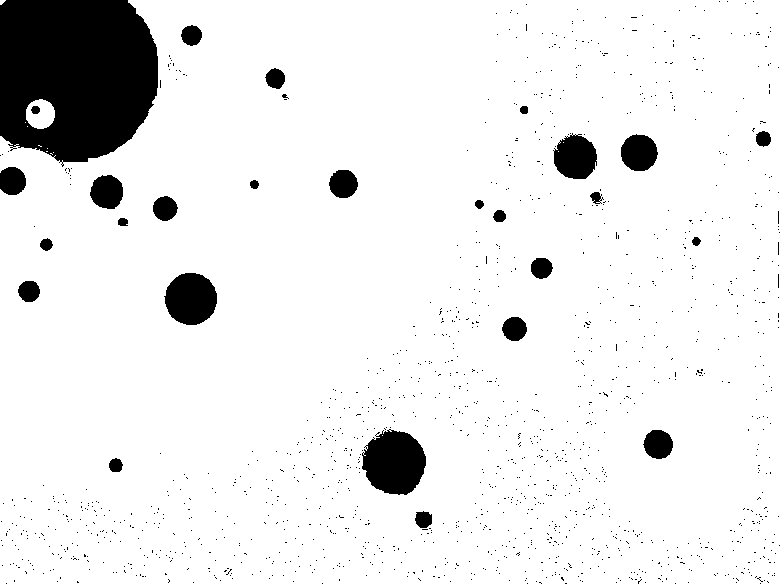
\includegraphics[width=\linewidth]{ballth}
			\caption{Foreground region}
		\end{subfigure}
		\hfill
		\centering
		\begin{subfigure}[h!]{0.45\linewidth}
			
			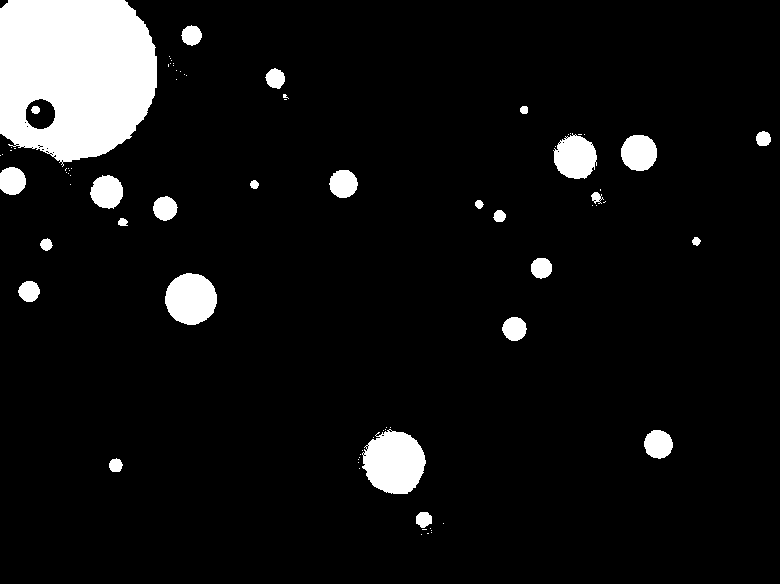
\includegraphics[width=\linewidth]{ballthl}
			\caption{foreground object region}
		\end{subfigure}%
		\caption{Min \& Max Filtered Images}
	\end{figure}
	\newpage
\end{document}
